\chapter{Resultados Experimentais}\label{CAP4}

O \textit{ip soft core} proposto possui duas grandes principais motivações: desempenho e precisão nas detecções de ataques \textit{DDoS}. Para isso foi feita a implementação do core a nível \textit{RTL(register-transfer level)}, seguido pela a síntese. Diante disso, é possível quantificar a utilização dos componentes do módulo dentro de uma \textit{FPGA} (descrição).As tabelas  mostram o relatório de utilização do artigo \cite{HOQUE201748} (um trabalho similar) e o trabalho proposto. 
\begin{table}[!htb]
	\centering
	\caption{Relatório de Utilização do artigo de comparação}
	\label{Tab:RUP}
	\begin{tabular}{lcccc}
		\hline
		\multicolumn{1}{c}{Tipo}&\multicolumn{1}{c}{Usado }&\multicolumn{1}{c}{Disponível}&\multicolumn{1}{c}{Utilização\%} \\ \midrule 
		
		CLB LUTs*&  1905  & 28800 & 0.60  \\   \midrule
		LUT as Logic & 1891  & 28800 &  0.60  \\  \midrule
		LUT as Memory &  14  & 7860 &  0.01  \\  \midrule
		LUT as Shift Register & 14  &  &   \\  \midrule
		CLB Registers  & 1131  & 28800 & 0.3  \\  \midrule
		Register as Flip Flop & 1255  & 2386  & 52    \\  \midrule
		Frequency &  118Mhz 
	\end{tabular}
\end{table}

A tabela \ref{Tab:RUP} traz o valores de alguns componentes da FPGA utilizada, mostrando estimativas de utilização, uma vez que é possível identificar através da síntese o que seria utilizado na placa escolhida, além de termos conhecimento  dos componentes disponíveis. Semelhantemente, A tabela \ref{Tab:RUAC} traz valores de utilização, porém para o módulo implementado nesse trabalho. Comparando as duas tabelas, podemos ver uma menor utilização dos componentes, no trabalho proposto. Além de uma maior frequência, o que garante uma detecção em um menor tempo.


\begin{table}[H]
	\centering
	\caption{Relatório de Utilização do trabalho proposto}
	\label{Tab:RUAC}
	\begin{tabular}{lcccc}
		\hline
		\multicolumn{1}{c}{Tipo}&\multicolumn{1}{c}{Usado }&\multicolumn{1}{c}{Disponível}&\multicolumn{1}{c}{Utilização\%} \\ \midrule
		
		CLB LUTs*&  1302  & 216960 & 0.60  \\   \midrule
		LUT as Logic & 1301  & 216960 &  0.60  \\  \midrule
		LUT as Memory &  1  & 99840 &  <0.01  \\  \midrule
		LUT as Shift Register & 1  &  &   \\  \midrule
		CLB Registers  & 1180  & 433920 & 0.27  \\  \midrule
		Register as Flip Flop & 1122  & 433920  &  0.26    \\  \midrule
		Frequency 120 MHZ
	\end{tabular}
\end{table}


Outro importante fator de validação do módulo seria o quão os valores se aproximam dos valores reais. Para isso, foi feito um \textit{TestBench} (um teste não sintetizável, no qual verifica o funcionamento, através de simulações) em \textit{systemverilog}. Foi comparado os valores adquiridos nos testes com valores calculados no \textit{Matlab}, com os devidos truncamentos das operações da figura ---.


\begin{table}[H]
	\centering
	\caption{Comparativo de resultados do Nahid implementado em software e hardware}
	\label{Tab:Tb}
	\begin{tabular}{lcccc}
		\hline
		\multicolumn{1}{c}{ Detecção}&\multicolumn{1}{c}{Matlab }&\multicolumn{1}{c}{Módulo}&\multicolumn{1}{c}{Erro (\%)}\\ \midrule
		
		1 (P1=365,P2=252,P3=953,D1=140,D2=200,D3=970)&0,82493 & 0,82812 & 1   \\   \midrule
		2 (P1=128,P2=515,P3=852,D1=130,D2=470,D3=970)&0,96874 & 0,96625 & 1.02    \\   \midrule
		3  (P1=150,P2=300,P3=853,D1=123,D2=340,D3=876)& 0,95585 & 0,95468  & 0.9  \\   \midrule	
		
	\end{tabular}
\end{table}

Na tabela \ref{Tab:Tb} as siglas P1,P2 e P3 são os vetores de perfil normal, já as siglas D1,D2 e D3, são os vetores que foram examinados. Podemos ver que mesmo que as taxas de erros são bem pequenas, o que mostra uma precisão considerável nos resultados do módulo. A figura \ref{simu}, mostra um exemplo de simulação nos seus últimos ciclos, vale a pena ressaltar, que com o \textit{threshold}, pode-se trazer a conclusão se existe um ataque ou não naquela para aqueles valores.

\begin{figure}[H]
	\centering
	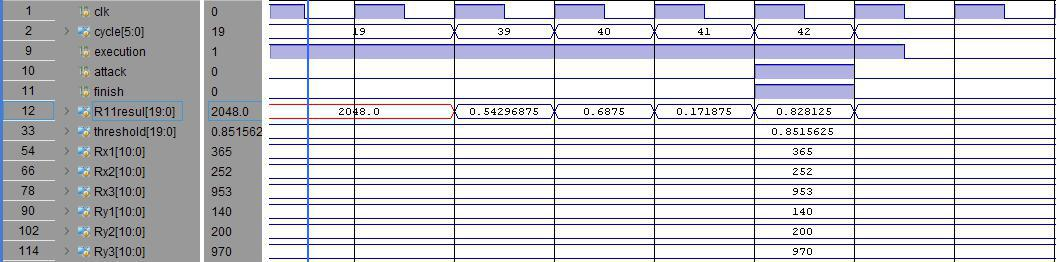
\includegraphics[width=12cm]{figures/simu.jpg}\\
	\caption{Simulação 1 da tabela  \ref{Tab:Tb}}
	\label{simu}
\end{figure}



\begin{table}[H]
	\centering
	\caption{Tempo de detecção}
	\label{Tab:TD}
	\begin{tabular}{lcccc}
		\hline
		\multicolumn{1}{c}{Detector}&\multicolumn{1}{c}{Artigo de comparação }&\multicolumn{1}{c}{Trabalho Proposto}&\multicolumn{1}{c}{Software(Matlab)}
		\\ \midrule
		
		Tempo de Detecção &  354 ns  &  350 ns & 296 $\mu$s  \\   \midrule
	
	\end{tabular}
\end{table}

A tabela \ref{Tab:TD} mostra que existe um pequeno ganho, desse trabalho em relação ao artigo de comparação (também implementado em hardware), e um ganho significativo em relação ao detector em software.

